
\chapter{Technical choice }

During this project we made a lot of technical choice. We will explain which choice we take and why.

\section{Type of communication}

First of all, we had to find the best way to integrate the simulator in \umld. Because we want to keep the possibility to change the simulator we have decided to put it outside. In this way, we had the possibility to change the simulator without changing everything in the plugin.

Moreover, we have to find the best way to realize the communication enter the simulator and the plugin. We decided to chose a socket communication, and send message only formatted as json object.

% A lot of type of communication inter process were suggested to create a discussion enter the plugin and the simulator. But we will present only the most consistent with their advantages and their drawbacks.

% The communication is the most important part of this project, because that will implement the interface between the two software.


\subsection{Socket}

This next table explain advantages and drawback of socket. We chose socket instead of other type of communication because it have a better ratio of Advantages/Drawback.
~\\

\begin{tabular}{|p{0.45\textwidth}||p{0.45\textwidth}|}
\hline
  \textbf{Advantages}&\textbf{Drawback}\\
\hline
Work with every simulator type (python, java, ...) & Message need to be formatted\\
\hline
& Not very fast\\
\hline
\end{tabular}

% \subsection{File}

% \begin{tabular}{|p{0.45\textwidth}||p{0.45\textwidth}|}
% \hline
%   \textbf{Advantages}&\textbf{Drawback}\\
% \hline
% Problem when two software want to change the same file at the same moment& Communication asynchronous\\
% \hline
% \end{tabular}

% \subsection{Named pipe}

% \begin{tabular}{|p{0.45\textwidth}||p{0.45\textwidth}|}
% \hline
%   \textbf{Advantages}&\textbf{Drawback}\\
% \hline
% It is possible to use the Simulator outside the graphical modeling tool & \\
% \hline
% \end{tabular}


% \subsection{Shared Memory}

% \begin{tabular}{|p{0.45\textwidth}||p{0.45\textwidth}|}
% \hline
%   \textbf{Advantages}&\textbf{Drawback}\\
% \hline
% It is possible to use the Simulator outside the graphical modeling tool & \\
% \hline
% \end{tabular}


% \subsection{Thread}

% \begin{tabular}{|p{0.45\textwidth}||p{0.45\textwidth}|}
% \hline
%   \textbf{Advantages}&\textbf{Drawback}\\
% \hline
% &problem if the thread don't avance at the good speed\\
% \hline
% \end{tabular}

% \subsection{Heritage}

% \begin{tabular}{|p{0.45\textwidth}||p{0.45\textwidth}|}
% \hline
%   \textbf{Advantages}&\textbf{Drawback}\\
% \hline
% Easy to implement&Need to add code in the simulator\\
% \hline
% &We can only use simulator in Java\\
% \hline
% \end{tabular}



% \subsection{Our solution}

% For this project we chose to use socket enter the plugin and the simulator. So we need to create a layer of communication for the simulator and a layer of communication for the plugin. Both layer will listen on a thread.

% The solution was not in this list of common way to communicate inter process. In fact, we use the \textit{Runtime} class which is in the java library.~\\

% \noindent
% \begin{tabular}{|p{0.45\textwidth}||p{0.45\textwidth}|}
% \hline
%   \textbf{Advantages}&\textbf{Drawback}\\
% \hline
% It is possible to use the Simulator outside the graphical modeling tool & \\
% \hline
% Work with every type of simulator& \\
% \hline
% \end{tabular}


\section{Type of message}

Now we have chosen that we will use socket to communicate enter the plugin and the simulator, we have too choose which type of object we will send by this socket.

In the same way, we list the type of message that we could send, and only three were relevant.

\begin{itemize}
\item String
\item Java object
\item Json message
\end{itemize}

Because String doesn't permit modularity and Java object require to use java for the simulator layer, we chose to use Json. Moreover, Json are send like String but with a formatted type.

To do that we use a library which permit to manipulate Json object in Java. We found it on Github \cite{json}.
~\\

Our json object are constructed like this:
~\\

plugin \overrightarrow{} simulator
\begin{lstlisting}[style=json]
  JsonPluginToSimulator = {
    initialize : boolean
    play : boolean
    stop : boolean
    restart : boolean
    random : boolean
    reload : boolean
    reloadPath : string
    state : string
  }
\end{lstlisting}

~\\

simulator \overrightarrow{} plugin
\begin{lstlisting}[style=json]
  JsonSimulatorToPlugin = {
    transitions : ["transition1", ...]
    error : boolean
    errorMessage : string
    currentClass : string
    currentStates : [
    {
      class : string
      instance : [
      {
        nom : string
        state : ["state1",...]
      }
      ...
      ]
    }
    ...
    ]
  }

\end{lstlisting}


\section{Overview of the project}

With this choice, it is possible to better understand how the project is construct. There is a plugin incorporate in \umld and a communication layer for the simulator. The plugin communicate to the communication layer with socket and json. The plugin receive the data send from the simulator, analyze them, display them, and send instruction to the simulator.

The figure \ref{fig:project} resume its.

\begin{figure}[h]
  \centering
  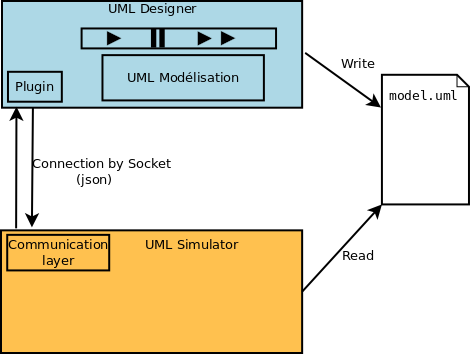
\includegraphics[width=\linewidth]{project}
  \caption{overview of the project}
  \label{fig:project}
\end{figure}



%%% Local Variables:
%%% mode: latex
%%% TeX-master: "../rapport_de_base"
%%% End:
